\documentclass[12pt,twocolumn,a4paper]{article}

\usepackage[a4paper,margin=0.72in,columnsep=0.29in]{geometry}
\usepackage{fontspec}
\setmainfont{Times New Roman}
\newfontfamily\bengalifont{Kalpurush}
\newcommand{\bn}[1]{{\bengalifont #1}}
\usepackage{setspace}
\singlespacing
\usepackage{microtype}
\usepackage{graphicx}
\usepackage{booktabs}
\usepackage{tabularx}
\usepackage{array}
\usepackage{enumitem}
\usepackage[table]{xcolor}
\usepackage{tikz}
\usetikzlibrary{arrows.meta,positioning,fit,calc,backgrounds}
\usepackage{caption}
\usepackage{titlesec}
\usepackage{hyperref}
\usepackage{xurl}
\usepackage{url}
\usepackage{placeins}
\usepackage{balance}
\usepackage{float}

\definecolor{medoraNavy}{HTML}{17365D}
\definecolor{medoraBlue}{HTML}{2D6CDF}
\definecolor{medoraTeal}{HTML}{138A8A}
\definecolor{medoraGreen}{HTML}{2E8B57}
\definecolor{medoraAmber}{HTML}{E09F3E}
\definecolor{medoraRed}{HTML}{C63C42}
\definecolor{medoraViolet}{HTML}{7251B5}
\definecolor{medoraGray}{HTML}{687386}

\hypersetup{
  colorlinks=true,linkcolor=medoraNavy,urlcolor=medoraBlue,citecolor=medoraTeal,
  pdftitle={Medora: Consent-Governed Clinical AI Infrastructure for Bangladesh},
  pdfauthor={Team Medora: Sarwad Hasan Siddiqui and Adiba Tahsin},
  pdfsubject={BCOLBD 2026 AI Category Whitepaper},
  pdfkeywords={clinical AI, consent, Bangladesh, safety benchmark, de-identification}
}
\captionsetup{font=normalsize,labelfont=bf,labelsep=period,skip=4pt}
\setlength{\parindent}{0pt}
\setlength{\parskip}{3.2pt}
\setlength{\emergencystretch}{2em}
\setlist[itemize]{leftmargin=1.1em,itemsep=1pt,topsep=2pt}
\setlist[enumerate]{leftmargin=1.25em,itemsep=1pt,topsep=2pt}
\titleformat{\section}{\bfseries\normalsize\color{medoraNavy}}{\thesection.}{0.45em}{}
\titleformat{\subsection}{\bfseries\normalsize\color{medoraNavy}}{\thesubsection}{0.45em}{}
\titlespacing*{\section}{0pt}{7pt}{2pt}
\titlespacing*{\subsection}{0pt}{5pt}{1pt}
\renewcommand{\refname}{References}

\newcolumntype{Y}{>{\raggedright\arraybackslash}X}
\tikzset{
  artifact/.style={draw=medoraNavy!72,rounded corners=3pt,minimum width=3.1cm,
    minimum height=1.35cm,align=center,inner sep=4pt},
  sys/.style={draw=medoraNavy!65,rounded corners=3pt,minimum height=1.05cm,
    align=center,inner sep=4pt},
  flow/.style={->,semithick,medoraNavy!76},
  measure/.style={draw=medoraNavy!55,rounded corners=3pt,minimum width=3.1cm,
    minimum height=1.05cm,align=center,inner sep=4pt},
  pipe/.style={draw=medoraNavy!60,rounded corners=3pt,minimum width=1.65cm,
    minimum height=1.05cm,align=center,font=\footnotesize}
}

\begin{document}

\twocolumn[
\begin{center}
{\bfseries Medora: Consent-Governed Clinical AI Infrastructure for Bangladesh}\par
\vspace{3pt}
{Team Medora: Sarwad Hasan Siddiqui and Adiba Tahsin}\par
{Department of Computer Science and Engineering, Khulna University of Engineering \& Technology}\par
{Supervision: Kazi Saeed Alam \quad $\cdot$ \quad BCOLBD 2026 AI Category}\par
{\url{https://medorahealth.vercel.app} \quad $\cdot$ \quad
\url{https://github.com/CSE-3200-System-Project/Medora}}\par
\vspace{5pt}
\color{medoraBlue}\rule{\textwidth}{1.2pt}
\end{center}
]

\begin{abstract}
A fluent language model can word clinical advice well, but fluency does not decide what patient
data it should see or how much its output is allowed to do. Medora pairs a deployed clinical
platform with a clear plan to test and prove that control layer in Bangladesh. Five named parts
keep the questions apart: how far the AI may act (\textbf{Arohon}), whether the safety line held
(\textbf{Lokkhon}), what consent costs in usefulness (\textbf{Shimana}), whether a fine-tuned
model stays safe enough to deploy (\textbf{Maya}), and a national drug-identity list
(\textbf{Akkhor}). Learned models handle speech, vision, and drafting; plain deterministic code
decides what is disclosed and what takes effect. Today's evidence is 134 privacy cases (94.7\%
precision, 75.5\% recall), 30 clinician-reviewed navigation fixtures (all seven emergencies kept
on both scored paths), 12 source-grounded summaries, and an index of 7,389 drugs and 67,001
brands. Arohon's tiers are specified; Shimana, Maya, and a learned de-identifier are registered
plans. Medora navigates and drafts for a clinician to approve. It does not diagnose, prescribe,
counsel, or claim to be a medical device.
\end{abstract}

\section{Problem and vision}

\textbf{Bangladesh needs useful digital health assistance without transferring clinical
authority to a general-purpose model.} Household out-of-pocket payments represented about
72.5\% of current health expenditure in 2022. WHO's Bangladesh page reports that medicines
and medical products accounted for 69.4\% of out-of-pocket payments in the 2015 national
accounts~\cite{wboop,whomedicines}. WHO identifies health-model risks
including inaccurate statements, automation bias, privacy loss, unequal access, and the
delegation of difficult choices to a model~\cite{wholmm}. These constraints require a
fluent Bengali response to be evaluated alongside enforceable controls.

\textbf{Bangladesh's new data regime turns that safety problem into an infrastructure
problem.} The Personal Data Protection Ordinance 2025 treats health information as
sensitive personal data. It defines valid consent as informed, specific, voluntary, and
affirmative. And it requires safeguards such as pseudonymisation, periodic risk assessment,
testing, and audit~\cite{pdpo}. Most provisions took immediate effect; selected
institutional and enforcement provisions commence on a later gazetted date after eighteen
months. Medora is an engineering tool for conformance, not a legal certificate; formal
certification stays with accredited bodies. What it adds is to make consent status and
data-sharing limits visible enough to test. The need is already official: in 2026 the Cabinet
Division warned every ministry, and Bangladesh Bank warned every bank, against sending
confidential data to third-party AI tools~\cite{cabinetai,bbai}. Medora's answer is a reusable
privacy layer, not a single application. Policy-before-inference, deny-by-default consent,
redaction, pseudonymisation, local-first routing, and audit are domain-agnostic components that
keep sensitive data inside the boundary and minimise what any external model can see. We build
and prove them in health, the hardest setting, as a reference implementation for a
privacy-aware, secure, AI-native Bangladesh whose same layer extends to any sector that holds
sensitive records.

\textbf{The gap is authority you can enforce in code.} A safe system needs the power to take
back a data-sharing grant, to hold the assistant to a fixed set of actions, to tie every answer
to a supplied record, and to save a booking with its audit trail together or not at all. Medora
therefore puts the policy check before the model and a human check after it. The thesis is short:
\emph{clinical AI should earn authority by risk class, consent, and evidence, not inherit it from
model confidence.}

\textbf{Objectives.} Medora will (i) formalise tiered authority, (ii) extend bilingual
safety and privacy evaluation, (iii) quantify the utility cost of narrower consent,
(iv) admit a locally deployable model only after red-flag and licence gates, and (v) keep
drug identity openly reusable. Deployed, measured, specified, and planned work remain
visually and verbally distinct.

\section{Use cases and existing solutions}

\textbf{Medora serves patients, doctors, and infrastructure adopters.} Patients use an
installable bilingual client to hold records, manage sharing, inspect access history, find
doctors, and book appointments. Doctors receive source-linked summaries and structured
drafts that remain editable before effect. A hospital, research group, or health-software
vendor can reuse the consent guard, benchmark runner, route registry, or medicine identity
layer independently of the Medora interface.

\begin{table*}[!t]
\caption{Publicly documented scope of representative systems. ``Outside reviewed scope''
limits the comparison to properties established in cited public material.}
\label{tab:comparison}
\centering
\renewcommand{\arraystretch}{1.02}
\setlength{\tabcolsep}{3pt}
\rowcolors{2}{white}{medoraNavy!7}
\begin{tabularx}{\textwidth}{@{}p{2.2cm}YYYYY@{}}
\toprule
System & Primary scope & Patient consent surface & Assistive-AI containment & Bangladesh drug identity & Public status \\
\midrule
OpenMRS & Modular EMR platform & Deployment-specific & Outside reviewed core scope & Deployment-supplied dictionaries & Mature open source~\cite{openmrs} \\
Bahmni & Hospital, laboratory, stock, billing & OpenMRS-based roles and workflow & Outside reviewed core scope & Deployment-supplied dictionaries & Open-source hospital suite~\cite{bahmni} \\
GNU Health & EMR, HMIS, public health, FHIR & Role/access facilities & Outside reviewed core scope & WHO essential medicines & Mature open source~\cite{gnuhealth} \\
Bangladesh SHR & National HIE, Health ID, longitudinal record & Citizen-controlled record sharing & Assistive-AI layer outside reviewed scope & National terminology registries & Government infrastructure~\cite{shr} \\
DocTime / Praava & Consultation, diagnostics, prescriptions & Product privacy controls & Conformance evidence outside reviewed scope & Service catalogues & Commercial services~\cite{doctime,praava} \\
Arogga & E-pharmacy and fulfilment & Transactional account controls & Conformance evidence outside reviewed scope & Large commercial catalogue & Commercial service~\cite{arogga} \\
\textbf{Medora} & Patient-held workflow plus research test bed & Purpose, provider, scope, validity, revocation, audit & Registry-bounded actions; source-linked drafts; local-first paths & 7,389 drugs; 67,001 brands & Live demo; MIT; archived v1.0.2~\cite{medoraarchive} \\
\bottomrule
\end{tabularx}
\end{table*}

\textbf{These systems are complementary.} OpenMRS, Bahmni, GNU Health, and the national SHR
cover broader hospital workflows and standards-based interoperability. Medora contributes
an inspectable boundary around assistive AI, coupled to Bangladesh medicine identity and
reproducible containment tests.

\begin{figure}[!t]
\centering
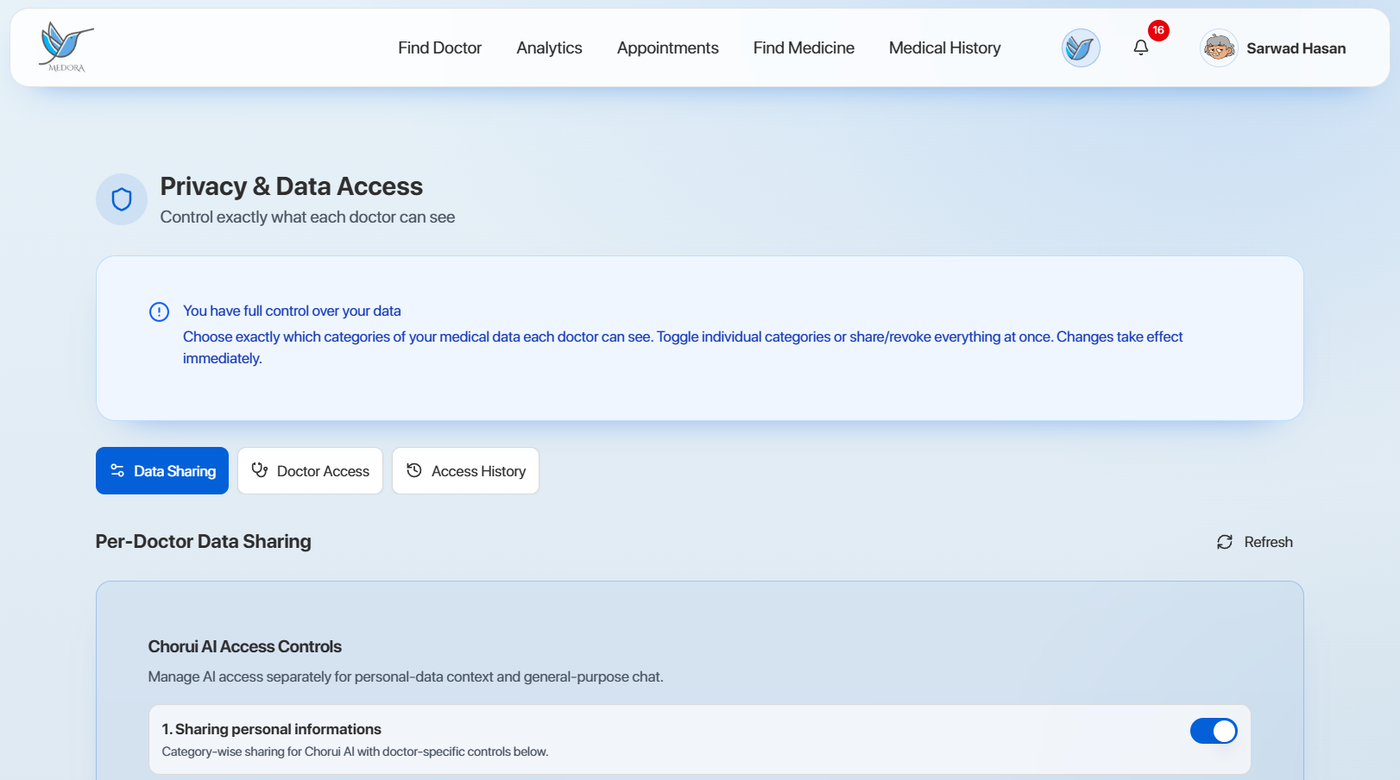
\includegraphics[width=\columnwidth]{../../softwarex/figures-ui/ui_consent_sharing.png}\\[3pt]
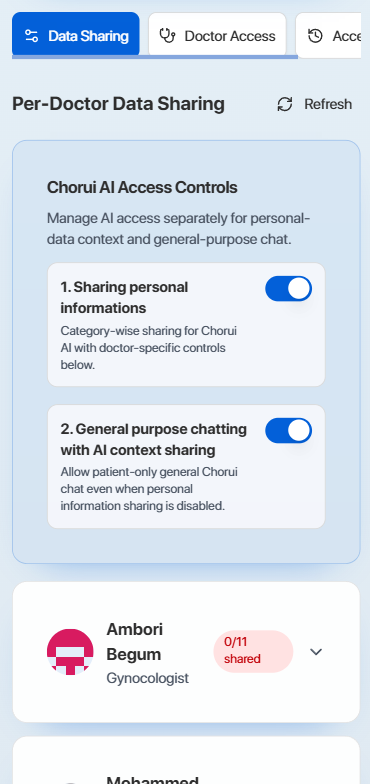
\includegraphics[width=.49\columnwidth]{../../softwarex/figures-ui/ui_mobile_consent.png}\hfill
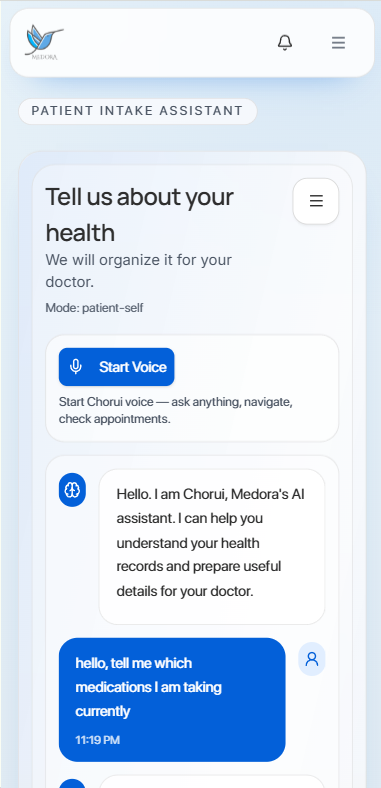
\includegraphics[width=.49\columnwidth]{../../softwarex/figures-ui/ui_mobile_assistant.png}
\caption{The deployed evidence surface: recipient/category sharing on desktop, the same
controls at a phone viewport, and the mobile patient-intake assistant. These interfaces
show that consent boundaries and assistive status are user-visible rather than policy prose
alone.}
\label{fig:ui}
\end{figure}

\section{The five-artifact framework}

\begin{figure*}[!t]
\centering
\begin{tikzpicture}[x=1cm,y=1cm,>=Latex]
  \node[draw=none,fill=medoraNavy,rounded corners=3pt,text=white,
        minimum width=5.0cm,minimum height=1.05cm,align=center,font=\bfseries] (core) at (0,0)
        {CONSENT ENGINE\\[-1pt]\normalfont\footnotesize deny by default $\cdot$ purpose $\cdot$ provider $\cdot$ scope};

  \node[artifact,fill=medoraBlue!9] (aro) at (-5.4,1.65)
        {\textbf{Arohon} (\bn{আরোহণ})\\[-1pt]\footnotesize \textbf{SPECIFIED} $\cdot$ authority tiers};
  \node[artifact,fill=medoraTeal!10,double] (lok) at (0,2.45)
        {\textbf{Lokkhon} (\bn{লক্ষণ})\\[-1pt]\footnotesize \textbf{MEASURED} $\cdot$ safety axes};
  \node[artifact,dashed,fill=medoraViolet!8] (shi) at (5.4,1.65)
        {\textbf{Shimana} (\bn{সীমানা})\\[-1pt]\footnotesize \textbf{PLANNED} $\cdot$ consent frontier};
  \node[artifact,dashed,fill=medoraAmber!13] (may) at (-3.25,-2.2)
        {\textbf{Maya} (\bn{মায়া})\\[-1pt]\footnotesize \textbf{PLANNED} $\cdot$ admission gate};
  \node[artifact,very thick,fill=medoraGreen!11] (uts) at (3.25,-2.2)
        {\textbf{Akkhor} (\bn{অক্ষর})\\[-1pt]\footnotesize \textbf{DEPLOYED} $\cdot$ drug identity};

  \foreach \n in {aro,lok,shi,may,uts}{\draw[->,semithick,medoraNavy!72] (core) -- (\n);}
  \node[font=\footnotesize,align=center,text=medoraGray] at (0,-3.25)
       {Status is written inside every node; border styles reinforce, but do not replace, the label.};
\end{tikzpicture}

\caption{Medora composes five artifacts around a deny-by-default consent engine.
Deployed means running in the platform; measured means archived results exist; specified
means design complete and scheduled for implementation; planned means a registered protocol
scheduled for execution. Each node prints its status explicitly.}
\label{fig:constellation}
\end{figure*}

\textbf{Each name maps to a technical function.} Arohon
(\bn{আরোহণ}, ``ascent'') specifies increasing authority; Lokkhon (\bn{লক্ষণ}, ``clinical
sign''; a homophone evoking \bn{লক্ষ্মণরেখা}, the line not to cross) tests what the system
must catch; Shimana
(\bn{সীমানা}, ``frontier'') will measure utility against disclosure; Maya (\bn{মায়া},
``illusion'') will test whether domain fluency preserves escalation sensitivity; and Akkhor (\bn{অক্ষর},
``character'') supplies canonical drug identity. Akkhor canonicalises, Arohon governs, Lokkhon tests,
Shimana prices, and Maya challenges the alternative.

\subsection{Arohon: graded autonomy}

\textbf{Arohon sets how far the AI may go as a ladder of tiers, capped by how dangerous the
case is.} In the specified execution order, an endpoint declares an intended tier; the policy engine resolves
actor, purpose, recipient, scopes, and risk class; the ceiling lowers the tier when needed;
and the selected tier is logged with the correlation identifier. Current routes already
provide deny-by-default consent, deterministic red flags, source-linked drafts, and human
confirmation; formal tier enums, ceilings, and tier logs are the specified next increment.

\begin{table}[!t]
\caption{Arohon authority tiers.}
\label{tab:tiers}
\centering
\small
\setlength{\tabcolsep}{3pt}
\rowcolors{2}{white}{medoraNavy!7}
\begin{tabularx}{\columnwidth}{@{}>{\raggedright\arraybackslash}p{2.35cm}>{\raggedright\arraybackslash}p{1.45cm}Y@{}}
\toprule
Tier / mode & Human gate & Constraint \\
\midrule
L0 Abstain & none & supported claims only \\
L1 Inform & reads & source-linked \\
L2 Suggest & confirms & before effect \\
L3 Escalate & acts & recall-first \\
L4 Break glass & notified & prior revocable grant \\
\bottomrule
\end{tabularx}
\end{table}

\begin{figure}[!t]
\centering
\resizebox{\columnwidth}{!}{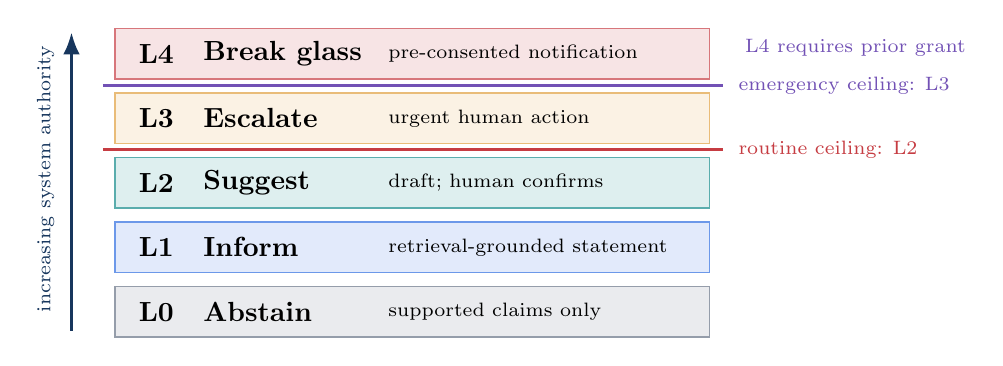
\begin{tikzpicture}[x=1cm,y=.82cm,>=Latex]
  \foreach \y/\tier/\name/\desc/\col in {
    0/L0/Abstain/supported claims only/medoraGray,
    1/L1/Inform/retrieval-grounded statement/medoraBlue,
    2/L2/Suggest/draft; human confirms/medoraTeal,
    3/L3/Escalate/urgent human action/medoraAmber,
    4/L4/Break glass/pre-consented notification/medoraRed}{
      \fill[\col!14] (0,\y) rectangle (7.55,\y+.78);
      \draw[\col!70,line width=.55pt] (0,\y) rectangle (7.55,\y+.78);
      \node[font=\bfseries,anchor=west] at (.18,\y+.39) {\tier};
      \node[font=\bfseries,anchor=west] at (1.0,\y+.39) {\name};
      \node[font=\scriptsize,anchor=west] at (3.35,\y+.39) {\desc};
  }
  \draw[very thick,medoraRed] (-.15,2.90) -- (7.72,2.90);
  \node[font=\scriptsize,fill=white,inner sep=1pt,anchor=west,text=medoraRed] at (7.88,2.90)
       {routine ceiling: L2};
  \draw[very thick,medoraViolet] (-.15,3.90) -- (7.72,3.90);
  \node[font=\scriptsize,fill=white,inner sep=1pt,anchor=west,text=medoraViolet] at (7.88,3.90)
       {emergency ceiling: L3};
  \node[font=\scriptsize,anchor=west,text=medoraViolet] at (7.88,4.48)
       {L4 requires prior grant};
  \draw[->,line width=1.1pt,medoraNavy] (-.55,.1) -- (-.55,4.72);
  \node[rotate=90,font=\scriptsize,text=medoraNavy] at (-.88,2.45) {increasing system authority};
\end{tikzpicture}
}
\caption{Authority rises from abstention to a pre-consented break-glass notification within
risk-specific ceilings. Risk policy determines the tier independently of model confidence.}
\label{fig:arohon}
\end{figure}

\textbf{Ceilings encode risk-specific authority.} Under the specification, routine queries
remain at L1--L2 and out-of-scope inputs fall to L0. Cardiac, stroke, anaphylaxis, and
obstetric red flags may surface an L3 emergency takeover, while L4 activates only with a
previously granted and still-valid notification recipient. The self-harm path is capped at
L3 in this proposal. It presents clinician-authored supportive text and time-aware
human-help options, excludes method content, and keeps dispatch under human control. This policy is a deliberate design
boundary for independent clinical and ethics review; it is an engineering specification
rather than a clinical guideline.

\textbf{Two traces make the specification testable.} ``Chest pain and difficulty
breathing'' maps to the cardiac risk class, pre-empts the model, and proposes a bilingual
L3 takeover with a one-tap emergency action; dismissal becomes a labelled false-positive
event. ``I do not want to live'' maps to the separate self-harm class, remains at L3, and
surfaces human support while preserving a manual choice. Both traces are finalist
implementation targets; the demo uses a mock number and a simulated emergency action.

\subsection{Architecture and infrastructure}

\textbf{Every AI request passes through one control point.} Medora comprises a Next.js
PWA, a FastAPI core, a separate FastAPI OCR service, and PostgreSQL. Its core exposes 21
assistive-AI endpoints in nine groups and authenticates
the actor and checks role, ownership or care relationship, appointment state, and consent.
External text, live audio, and cloud OCR are different recipients with different grants.
Local Whisper, YOLO, and PaddleOCR remain within the deployment, so local mode stays local.

\begin{figure*}[!t]
\centering
\resizebox{.80\textwidth}{!}{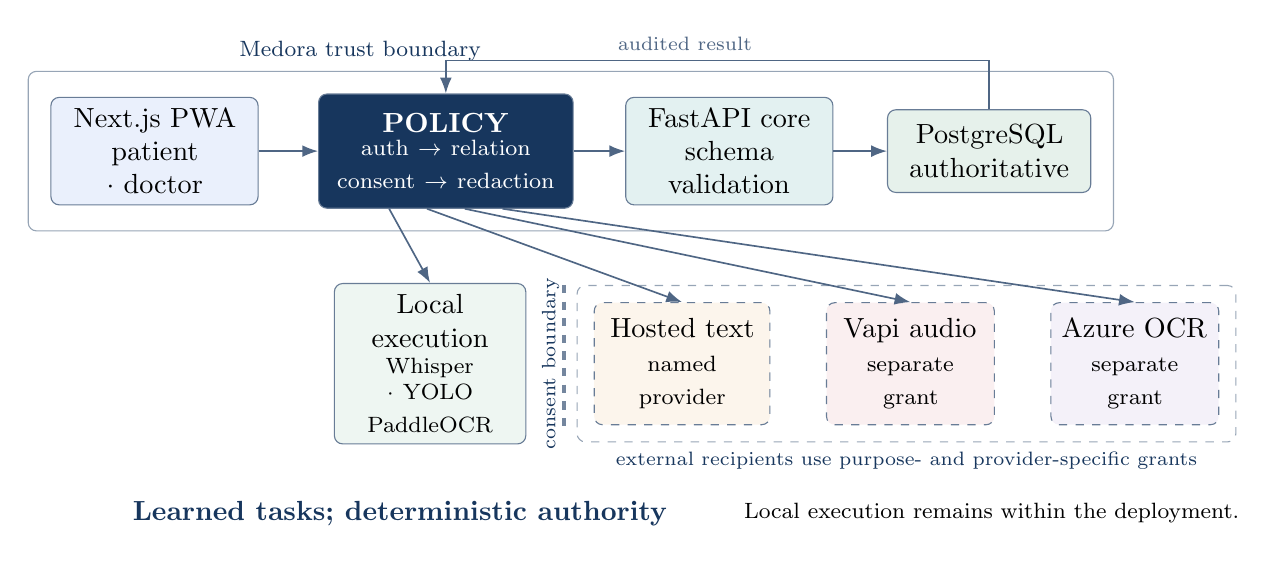
\begin{tikzpicture}[x=1cm,y=1cm,>=Latex]
  % Explicit text width on every top-row node (instead of only minimum width) so
  % each box has a fixed, predictable footprint and cannot auto-grow into its
  % neighbour; node centres are spaced with a clear margin beyond each half-width.
  \node[sys,fill=medoraBlue!10,text width=2.35cm,align=center] (pwa) at (-6.75,1.25)
       {Next.js PWA\\patient $\cdot$ doctor};
  \node[sys,fill=medoraNavy,text=white,text width=2.95cm,align=center,minimum height=1.45cm]
       (policy) at (-3.05,1.25)
       {\textbf{POLICY}\\[-1pt]\footnotesize auth $\rightarrow$ relation\\consent $\rightarrow$ redaction};
  \node[sys,fill=medoraTeal!12,text width=2.35cm,align=center] (api) at (.55,1.25)
       {FastAPI core\\schema validation};
  \node[sys,fill=medoraGreen!12,text width=2.30cm,align=center] (db) at (3.85,1.25)
       {PostgreSQL\\authoritative};

  \draw[flow] (pwa) -- (policy);
  \draw[flow] (policy) -- (api);
  \draw[flow] (api) -- (db);
  \draw[flow] (db.north) -- ++(0,.62) -| node[pos=.28,above,font=\scriptsize]{audited result} (policy.north);

  \node[sys,fill=medoraGreen!8,text width=2.15cm,minimum height=1.55cm] (local) at (-3.25,-1.45)
       {Local execution\\\footnotesize Whisper $\cdot$ YOLO\\PaddleOCR};
  \node[sys,dashed,fill=medoraAmber!10,text width=1.95cm,minimum height=1.55cm] (text) at (-.05,-1.45)
       {Hosted text\\\footnotesize named provider};
  \node[sys,dashed,fill=medoraRed!8,text width=1.85cm,minimum height=1.55cm] (audio) at (2.85,-1.45)
       {Vapi audio\\\footnotesize separate grant};
  \node[sys,dashed,fill=medoraViolet!8,text width=1.85cm,minimum height=1.55cm] (ocr) at (5.70,-1.45)
       {Azure OCR\\\footnotesize separate grant};

  \draw[flow] ([xshift=-.72cm]policy.south) -- (local.north);
  \draw[flow] ([xshift=-.24cm]policy.south) -- (text.north);
  \draw[flow] ([xshift=.24cm]policy.south) -- (audio.north);
  \draw[flow] ([xshift=.72cm]policy.south) -- (ocr.north);

  \begin{pgfonlayer}{background}
    \node[draw=medoraNavy!45,rounded corners=3pt,fit=(pwa)(policy)(api)(db),
          inner sep=8pt,label={[font=\footnotesize,text=medoraNavy]above left:Medora trust boundary}] {};
  \end{pgfonlayer}
  \begin{pgfonlayer}{background}
    \node[draw=medoraNavy!45,dashed,rounded corners=3pt,fit=(text)(audio)(ocr),inner sep=6pt,
          label={[font=\scriptsize,text=medoraNavy]below:external recipients use purpose- and provider-specific grants}] (external) {};
  \end{pgfonlayer}
  \draw[dashed,very thick,medoraNavy!60] (-1.55,-.45) -- (-1.55,-2.28);
  \node[font=\scriptsize,text=medoraNavy,rotate=90] at (-1.72,-1.45)
       {consent boundary};
  \node[font=\bfseries,text=medoraNavy,anchor=west] at (-7.15,-3.35)
       {Learned tasks; deterministic authority};
  \node[font=\footnotesize,anchor=east] at (7.15,-3.35)
       {Local execution remains within the deployment.};
\end{tikzpicture}
}
\caption{Control flow and trust boundaries. Every inference path passes through the policy
chokepoint; PostgreSQL remains authoritative after reconnect and external recipients are
separately consented.}
\label{fig:architecture}
\end{figure*}

\textbf{Learned components perceive and draft; deterministic code decides authority.}
Speech transcription, prescription-region detection, OCR, and hosted text generation use
learned models. Consent resolution, redaction, pseudonymisation, intent normalisation,
role-scoped route lookup, specialty and medicine matching, emergency rules, dosage grammar,
and structured parsing remain inspectable code paths. The orchestrator sanitises every level
of its input and replaces stable subject identifiers with a random per-request correlation ID.
It then validates the output against a schema and records only provider and latency metadata;
raw prompts and findings stay out of the default logs. Chorui's immutable registry contains 24 entries over 23 intents: 11 patient,
11 clinician, and two shared; administrative routes remain outside its scope. Table~\ref{tab:aimethods}
makes training, inference, evaluation, and status explicit.

\begin{table*}[!t]
\caption{AI and algorithm inventory. ``Deployed option'' means the path exists in the live
stack and may require configuration or a separate grant; planned rows identify registered
evaluation work.}
\label{tab:aimethods}
\centering
\scriptsize
\renewcommand{\arraystretch}{1.03}
\setlength{\tabcolsep}{1.5pt}
\rowcolors{2}{white}{medoraNavy!7}
\begin{tabularx}{\textwidth}{@{}>{\raggedright\arraybackslash}p{1.35cm}>{\raggedright\arraybackslash}p{2.25cm}>{\raggedright\arraybackslash}p{2.25cm}>{\raggedright\arraybackslash}p{1.40cm}>{\raggedright\arraybackslash}p{1.40cm}>{\raggedright\arraybackslash}p{2.25cm}Y@{}}
\toprule
Task & Model / algorithm & Data source & Train / infer & Status & Evaluation & Safety boundary \\
\midrule
Dictation & faster-whisper, Whisper small & consented live clinician audio & pretrained; local inference & Deployed option & workflow and route tests & local processing; editable draft \\
Live voice & Vapi tool bridge & separately consented audio & provider inference & Deployed option & route and guard tests & separate recipient grant; same registry \\
Region detection & project-trained YOLO ONNX & private student-project prescription images & local training; local inference & Deployed prototype & workflow evaluation; clinical study scheduled & regions remain non-authoritative \\
OCR & PaddleOCR / Azure Document Intelligence & prescription or report image & pretrained; local or cloud inference & Deployed options & review-gated prototype; clinical study scheduled & row confirmation; cloud grant separate \\
Text drafting & Groq GPT-OSS-120B default; Gemini, Cerebras, mock & redacted task payload and authorised record subset & provider inference & Deployed options & 12 source-accounting fixtures; schema tests & policy precedes model; backend attaches sources \\
Drug matching & trigram, edit distance, dosage grammar & Akkhor corpus & rules; local inference & Deployed & reproducible corpus counts & candidates only; clinician confirms OCR rows \\
Navigation & registry, synonyms, fuzzy/similarity matching & curated intents, specialties, red-flag rules & rules; local inference & Measured & 30 reviewed fixtures; 7/7 emergency labels retained; 5 conservative escalations & red flags pre-empt generation; manual browse remains \\
PHI redaction & bilingual patterns and pseudonymisation & 134 synthetic production-path cases & rules; local inference & Measured & P 94.7\%, R 75.5\%, over-redaction 3.2\% & measured baseline informs recall upgrade \\
PHI span recognition & MuRIL / XLM-R; BanglaBERT research comparator~\cite{muril,xlmr,banglabert} & planned 8k--15k synthetic Bengali, English, romanised cases; existing 134 held out & token-classifier fine-tuning planned & Planned & rules vs model vs union; P/R/F1, over-redaction, CPU latency, 3 seeds & recall-first threshold; ONNX feature flag; licence gate \\
Maya gate & TigerLLM-1B candidate with LoRA~\cite{tigerllm} & redistributable, de-identified Bangla dialogue; corpus selection scheduled & fine-tuning planned & Planned & escalation sensitivity on reviewed red flags plus benign controls and CIs & admission gate precedes deployment; tier remains policy-set \\
\bottomrule
\end{tabularx}
\end{table*}

\textbf{Human authority is structural.} Summaries are read-only and receive source
references from the backend after validation, constraining source references to supplied identifiers.
Specialty search returns candidates beside manual browsing. Consultation outputs pre-fill
forms a doctor edits and signs. OCR rows carry
\texttt{authoritative\_writeback=false} and require row-level confirmation. Medora's role
is navigation, reviewed drafting, and non-authoritative extraction.

\textbf{Administrative authority is scoped, not global.} The deployed platform authorises
administration through a single role; the specified stewardship layer binds each
administrator to an affiliation, so authority becomes a scope multiplied by a permission set.
A central administrator keeps platform-wide control and is the only role that can create other
administrators. An organisation administrator sees only the doctors, appointments, and records
of its own hospital or clinic, and a facility administrator is limited to one branch. A separate
data-protection role can read consent and audit records but holds no operational control. Because the ordinance makes a hospital
the data controller for its patients, the organisation scope makes that boundary observable
and testable. Every privileged action joins an administrative audit beside the existing
patient-access log, destructive actions require a second administrator, and emergency
elevation follows the L4 break-glass rule and is logged. The same audit already lets a patient
inspect who accessed a record and extends toward the ordinance's export and erasure rights.
Scoped roles, the affiliation model, and time-boxed delegated grants are specified over the
deployed flat-admin controls.

\textbf{Transactional and database controls cover non-model execution paths.} Appointment
creation locks the idempotency key and slot, then commits the appointment, replay result,
audit entry, and outbox event together; a unique active-slot constraint is the final guard.
Across 30 fresh-slot repetitions at each of 2, 10, and 50 concurrent attempts, all 90 trials
preserved exactly one commit. Transaction p95 was 38.8/580.8/1,571.5 ms and outbox-processing
p95 was 67.7/696.0/1,520.9 ms. These fixture results establish contention behavior under the
reported test envelope. Events publish after commit and reconnecting clients re-query PostgreSQL. A release
audit also found anonymous database grants with row-level security disabled. The release
revoked the grants, enabled deny-by-default RLS, restricted direct subscriptions to a
trigger-maintained feed, pinned trigger search paths, and added negative access tests.
The archived v1.0.2 receipt records passing backend, AI-service, integration, security,
container, and frontend gates; all 12 English/Bengali browser specifications executed their
authenticated journeys~\cite{medoraarchive}.

\section{Evaluation and research plan}

\subsection{Shimana: planned consent--utility frontier}

\textbf{Shimana asks a measurable question: how does task utility change as disclosure is
broadened?} A fixed bilingual task set will run under five configurations: local only (L), local
plus Akkhor (L+K), a redacted record subset (L+K+R), a hosted model under a matching grant
(L+K+R+H), and an offline, de-identified unrestricted research control (U). Utility comprises specialty-navigation
agreement, summary source-accounting, and medicine-match precision. Privacy exposure is
undetected PHI spans per 1,000 requests. The reporter will emit paired results, bootstrap confidence
intervals, the non-dominated set, and a knee estimate.

\begin{figure*}[!t]
\centering
\resizebox{.70\textwidth}{!}{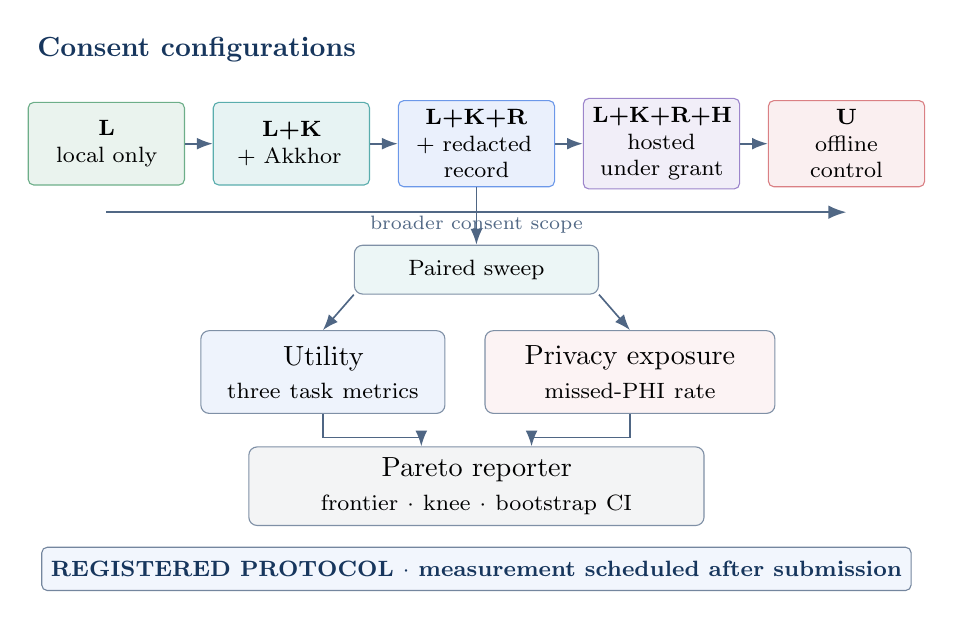
\begin{tikzpicture}[x=1cm,y=1cm,>=Latex]
  \node[font=\bfseries,text=medoraNavy,anchor=west] at (-1.0,2.75) {Consent configurations};
  \node[draw=medoraGreen!70,fill=medoraGreen!10,rounded corners=2pt,text width=1.75cm,
        minimum height=1.05cm,align=center,font=\footnotesize] (cfgL) at (0,1.55)
        {\textbf{L}\\local only};
  \node[draw=medoraTeal!70,fill=medoraTeal!10,rounded corners=2pt,text width=1.75cm,
        minimum height=1.05cm,align=center,font=\footnotesize] (cfgK) at (2.35,1.55)
        {\textbf{L+K}\\+ Akkhor};
  \node[draw=medoraBlue!70,fill=medoraBlue!10,rounded corners=2pt,text width=1.75cm,
        minimum height=1.05cm,align=center,font=\footnotesize] (cfgR) at (4.70,1.55)
        {\textbf{L+K+R}\\+ redacted record};
  \node[draw=medoraViolet!70,fill=medoraViolet!10,rounded corners=2pt,text width=1.75cm,
        minimum height=1.05cm,align=center,font=\footnotesize] (cfgH) at (7.05,1.55)
        {\textbf{L+K+R+H}\\hosted under grant};
  \node[draw=medoraRed!65,fill=medoraRed!8,rounded corners=2pt,text width=1.75cm,
        minimum height=1.05cm,align=center,font=\footnotesize] (cfgU) at (9.40,1.55)
        {\textbf{U}\\offline control};
  \foreach \a/\b in {cfgL/cfgK,cfgK/cfgR,cfgR/cfgH,cfgH/cfgU}{\draw[flow] (\a)--(\b);}
  \draw[->,line width=.8pt,medoraNavy!75] (0,.68) -- (9.40,.68)
       node[midway,below,font=\scriptsize,fill=white,inner sep=1pt]{broader consent scope};

  \node[measure,fill=medoraTeal!8,text width=1.9cm,minimum height=.62cm,font=\footnotesize]
       (sweep) at (4.70,-.05) {Paired sweep};
  \node[measure,fill=medoraBlue!8,text width=2.6cm] (utility) at (2.75,-1.35)
       {Utility\\\footnotesize three task metrics};
  \node[measure,fill=medoraRed!6,text width=3.4cm] (privacy) at (6.65,-1.35)
       {Privacy exposure\\\footnotesize missed-PHI rate};
  \node[measure,fill=medoraGray!8,text width=5.5cm,minimum height=.82cm] (report) at (4.70,-2.80)
       {Pareto reporter\\\footnotesize frontier $\cdot$ knee $\cdot$ bootstrap CI};
  \draw[flow] (cfgR.south) -- (sweep.north);
  \draw[flow] (sweep.south west) -- (utility.north);
  \draw[flow] (sweep.south east) -- (privacy.north);
  \draw[flow] (utility.south) -- ++(0,-.30) -| ([xshift=-.70cm]report.north);
  \draw[flow] (privacy.south) -- ++(0,-.30) -| ([xshift=.70cm]report.north);
  \node[draw=medoraNavy!60,fill=medoraBlue!6,rounded corners=2pt,
        minimum width=9.2cm,minimum height=.55cm,font=\footnotesize\bfseries,
        text=medoraNavy] at (4.70,-3.85)
       {REGISTERED PROTOCOL $\cdot$ measurement scheduled after submission};
\end{tikzpicture}
}
\caption{Registered Shimana experiment. The diagram fixes interventions, paired metrics,
and reporting outputs; execution is scheduled after submission.}
\label{fig:shimana}
\end{figure*}

\subsection{Lokkhon: measured safety baselines}

\textbf{Lokkhon publishes sample size beside every metric.} Its status is measured for
axes A--C, pilot (n=4) for D, and planned for E. Axis A tests red-flag
escalation; B tests indirect prompt injection; C tests identifier leakage and
over-redaction; D tests romanised code-mixing; and E will measure calibrated abstention with
a risk--coverage curve. The current harness archives machine-readable cases, exclusion and
outcome accounting, mock/live separation, and bootstrap reporters.

\begin{figure}[!t]
\centering
\resizebox{\columnwidth}{!}{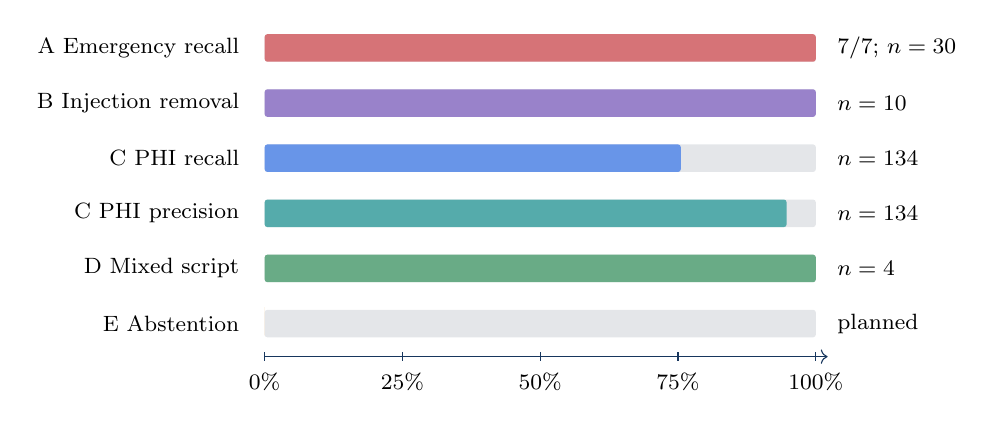
\begin{tikzpicture}[x=1cm,y=.7cm]
  \def\bar#1#2#3#4#5{%
    \node[anchor=east,font=\footnotesize] at (0,#1) {#2};
    \fill[medoraGray!18,rounded corners=1pt] (0.2,#1-.25) rectangle (7.2,#1+.25);
    \fill[#4!72,rounded corners=1pt] (0.2,#1-.25) rectangle ({0.2+7*#3/100},#1+.25);
    \node[anchor=west,font=\footnotesize] at (7.35,#1) {#5};
  }
  \bar{5}{A Emergency recall}{100}{medoraRed}{7/7; $n=30$}
  \bar{4}{B Injection removal}{100}{medoraViolet}{$n=10$}
  \bar{3}{C PHI recall}{75.5}{medoraBlue}{$n=134$}
  \bar{2}{C PHI precision}{94.7}{medoraTeal}{$n=134$}
  \bar{1}{D Mixed script}{100}{medoraGreen}{$n=4$}
  \bar{0}{E Abstention}{0}{medoraAmber}{planned}
  \draw[->,medoraNavy] (.2,-.6) -- (7.35,-.6);
  \foreach \x/\t in {.2/0,1.95/25,3.7/50,5.45/75,7.2/100}{
    \draw[medoraNavy] (\x,-.52)--(\x,-.68);
    \node[font=\footnotesize,anchor=north] at (\x,-.72) {\t\%};
  }
\end{tikzpicture}
}
\caption{Current Lokkhon baselines. Axis D is an explicitly labelled four-case pilot; axis
E is scheduled for the next benchmark release.}
\label{fig:lokkhon}
\end{figure}

\textbf{The current results establish containment baselines.} The
privacy suite contains 134 synthetic production-path cases and yields 94.7\% span precision,
75.5\% recall, 3.2\% over-redaction, and 43 documented boundary notes. Extended rules for the
leaking classes (unlabelled and cued names, obfuscated emails, textual dates, bare IDs,
addresses) now redact every annotated span on this development set at 96.9\% precision and
2.4\% over-redaction. Since those rules were tuned on that set, a held-out probe of novel
identifiers is the honest test: structured and cued classes generalise; the residual narrows
to unlabelled, unseen names. The reviewed navigation
set contains 30 fixtures: all seven emergency labels were recorded on both scored paths,
with complete emergency-label retention and five conservative escalations. A licensed reviewer changed
two authored Bengali labels to emergency before the rules were frozen. Twelve summary
fixtures account for every backend-supplied source under the deterministic mock. These
constructed sets establish a reproducible baseline for broader population evaluation.

\textbf{Prescription OCR remains a review-gated prototype.} The handwriting pipeline supports
workflow integration while clinical-accuracy evaluation awaits an independently adjudicated
corpus. The student-project image set stays private, since its permission covered project use
rather than public redistribution. Every extracted row is non-authoritative and needs
clinician confirmation, so we report workflow status and the next validation step, not an
accuracy percentage.

\subsection{Planned learned PHI recognition}

\textbf{The first post-submission build advances the measured redaction baseline.} The
residual after the extended rules is unlabelled, previously unseen names in both scripts, which
pattern rules cannot generalise to; recognising unseen names is exactly what a learned model
does. A reproducible generator will create 8,000--15,000 Bengali, English, and romanised
sentences, including hard negatives. Each sentence is BIO-tagged for names, clinicians, phones,
NIDs, addresses, dates, ages at least 90, hospitals, email, and medical-record numbers. MuRIL and XLM-R
are deployment candidates; BanglaBERT is retained only as a research comparator because its
published licence is non-commercial. The existing 134 cases remain untouched as a held-out
test. Across three seeds, rules, each model, and a recall-first union will report span
precision, recall, F1, false-redaction rate, bootstrap intervals, and CPU latency. Only a
licence-cleared ONNX model that improves recall within the predefined over-redaction limit
can enter the platform behind a feature flag. This registered build and evaluation plan
defines the release gate.

\subsection{Maya: planned model-admission gate}

\textbf{Maya turns escalation sensitivity into a deployment admission test.} The hypothesis is
that non-emergency dialogue can teach a small model to reassure when escalation is required.
TigerLLM-1B is the current candidate; final selection follows the licence and corpus review.
LoRA tuning would use a
redistributable, de-identified Bangla dialogue corpus after translation, licence, and ethics
review. The frozen comparison will score the base and tuned model on the clinician-reviewed
red-flag set plus 25--30 benign controls. Primary outcome is first-sentence escalation
sensitivity with a confidence interval; benign false-alarm rate detects trivial always-alert
behaviour. Self-harm cases use a separate agency-preserving rubric. Deployment admission
requires passing the gate, while Arohon continues to select the tier. Corpus selection,
adapter training, and archival execution are scheduled, so the paper reports the protocol.

\section{Risk management and validation scope}

\textbf{The team tracks risk as an engineering artifact.} Table~\ref{tab:risks}
distinguishes deployed controls from research commitments and pairs each initial risk with
a residual band and next validation step. Consent revocation governs future disclosure;
75.5\% recall is the baseline for the planned union recogniser; and seven reviewed
emergencies anchor expansion of clinical coverage.

\begin{table*}[!t]
\caption{Risk register. Evidence refers to the current release; P denotes a planned 2.0
control. H/M/L are qualitative impact or residual-risk bands, not probabilities.}
\label{tab:risks}
\centering
\renewcommand{\arraystretch}{.98}
\setlength{\tabcolsep}{1.5pt}
\rowcolors{2}{white}{medoraNavy!7}
\begin{tabularx}{\textwidth}{@{}>{\raggedright\arraybackslash}p{3.55cm}>{\raggedright\arraybackslash}p{7.70cm}Y@{}}
\toprule
Risk (initial $\rightarrow$ residual) & Control & Current evidence / next step \\
\midrule
Clinical-advice accuracy (H$\rightarrow$M) & deterministic red flags; drafts only; P Arohon ceilings & 30 reviewed fixtures; P tier logs \\
PHI exposure (H$\rightarrow$M) & deny-by-default grant; rule redaction; P union span recogniser & 134 cases; 75.5\% recall baseline \\
Consent alignment (H$\rightarrow$L--M) & purpose, provider, scope, version, validity, revocation & unit and integration tests \\
Administrative privilege/scope (M$\rightarrow$L--M) & P scoped roles; two-person destructive actions; admin audit; logged L4 break-glass & deployed flat admin; affiliation scoping specified \\
Indirect prompt injection (H$\rightarrow$M) & typed schema; out-of-band registry and policy & 10/10 cases removed \\
Source grounding (H$\rightarrow$M) & source attachment; Akkhor grounding; L0 abstention & 12 summary fixtures; axis E scheduled \\
Escalation sensitivity (H$\rightarrow$M) & model-independent emergency tier; P Maya admission gate & registered protocol \\
OCR extraction quality (H$\rightarrow$M) & non-authoritative output; mandatory confirmation & clinical evaluation scheduled \\
Provider continuity/retention (M$\rightarrow$M) & provider abstraction; local paths; retention manifest & manifest present \\
Emergency-service continuity (H$\rightarrow$M) & time-aware registry; manual alternatives & P health checks \\
Cost scaling (M$\rightarrow$L--M) & deterministic routing; caching; batch; spend caps & planning envelope \\
Clinician adoption (H$\rightarrow$H) & editable drafts; patients free; physician-workflow pilot & pilot scheduled \\
Banglish/code-mix robustness (M$\rightarrow$M) & transliteration-aware cases and encoders & four-case pilot; expansion scheduled \\
Dataset licence compatibility (H$\rightarrow$M) & per-source provenance; research/deployment licence gate & corpus selection scheduled \\
Clinician review capacity (M$\rightarrow$M) & publish adjudicated samples; version benchmark & reviewer capacity determines scale \\
\bottomrule
\end{tabularx}
\end{table*}

\section{Akkhor, feasibility, and distribution}

\begin{table*}[!t]
\caption{Monthly infrastructure scenarios in US dollars. The 1,000-MAU column starts from
the repository deployment estimate; higher Azure columns use linear scaling as a
conservative stress assumption. Text assumes three calls/MAU, 1,000 input
and 250 output tokens/call at current Groq GPT-OSS-120B rates~\cite{groq}.}
\label{tab:cost}
\centering
\scriptsize
\setlength{\tabcolsep}{3pt}
\rowcolors{2}{white}{medoraNavy!7}
\begin{tabularx}{\textwidth}{@{}p{3.15cm}rrrY@{}}
\toprule
Line item & 1k MAU & 10k MAU & 100k MAU & Basis / unresolved variable \\
\midrule
Backend containers and registry & 20--35 & 200--350 & 2,000--3,500 & current FastAPI container plus Azure registry estimate \\
OCR: local container + cloud & 30--100 & 300--1,000 & 3,000--10,000 & local PaddleOCR/YOLO plus usage-dependent Document Intelligence \\
PostgreSQL and auth & 25 & 25--75 & 25--125 & Supabase Pro starts at US\$25; compute upgrades are usage-dependent~\cite{supabasepricing} \\
Groq text inference & 0.90 & 9.00 & 90.00 & uncached input US\$0.15/M; output US\$0.60/M \\
Cached or batch text case & 0.45--0.68 & 4.50--6.75 & 45.00--67.50 & eligible-text alternative shown separately from totals \\
Monitoring & 0--10 & 10--50 & 50--200 & telemetry and retention determine the tier \\
Staffed support & Pilot & Pilot & Pilot & tickets and clinician onboarding measured in pilot \\
Subtotal before support & 75.90--170.90 & 544--1,484 & 5,165--13,915 & tax, FX, optional Vapi audio, and support listed separately \\
With 20\% contingency & 91.08--205.08 & 652.80--1,780.80 & 6,198--16,698 & contingency applies to priced rows only \\
Infrastructure / paying doctor & 1.82--4.10 & 1.31--3.56 & 1.24--3.34 & assumes 20 active patients per paying doctor; excludes support \\
\bottomrule
\end{tabularx}
\end{table*}

\textbf{Akkhor is reusable Bangladesh drug infrastructure rather than an application
feature.} A reproducible script reconciles five published datasets into immutable canonical
drug identities keyed by generic, strength, and form; commercial brands map many-to-one;
and a trigram index supports typo-tolerant lookup. The loaded release contains 71,795 source
rows, 7,389 canonical drugs, 67,001 brand entries, 74,390 search terms, 5,242 distinct
generics, and 52,117 distinct brands. Provenance is preserved per source. Current validation
covers reproducible identity construction; regulator review and indication validation are
future work.

\begin{figure*}[!t]
\centering
\resizebox{.72\textwidth}{!}{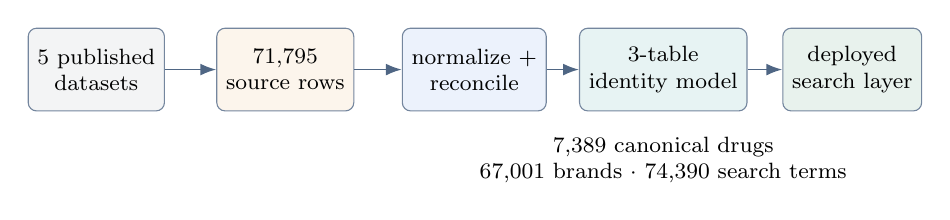
\begin{tikzpicture}[x=1cm,y=1cm,>=Latex]
  \node[pipe,fill=medoraGray!8] (src) at (0,0) {5 published\\datasets};
  \node[pipe,fill=medoraAmber!10] (rows) at (2.4,0) {71,795\\source rows};
  \node[pipe,fill=medoraBlue!9] (norm) at (4.8,0) {normalize +\\reconcile};
  \node[pipe,fill=medoraTeal!10] (tables) at (7.2,0) {3-table\\identity model};
  \node[pipe,fill=medoraGreen!11] (api) at (9.6,0) {deployed\\search layer};
  \foreach \a/\b in {src/rows,rows/norm,norm/tables,tables/api}{\draw[flow] (\a)--(\b);}
  \node[font=\footnotesize,align=center] at (7.2,-1.15)
       {7,389 canonical drugs\\67,001 brands $\cdot$ 74,390 search terms};
\end{tikzpicture}
}
\caption{Akkhor turns five source datasets into canonical identity and a deployed platform
search layer. The counts are generated from the current loaded corpus.}
\label{fig:akkhor}
\end{figure*}

\textbf{Akkhor stays free; revenue comes from workflow, hosting, and conformance, never from
the open assets.} Application code is MIT-licensed and the compiled medicine corpus is CC BY
4.0, so neither Akkhor nor patient access is ever a paid line. The open core instead supports
four service streams. A chamber and clinic subscription sells the clinician workflow; the
value proposition is less clerical time, with a design target of two minutes saved across 30
daily consultations. An institution stream sells on-premise deployment on a privacy premium
with support. A conformance stream offers Lokkhon-based safety testing and consent-conformance
review to other applications that must demonstrate PDPO handling. This reuses the benchmark and
never touches the free dataset. The same in-boundary stack also reaches adjacent
public-sector and financial deployments, the market opened by the 2026 government cautions
noted in Section~1. Table~\ref{tab:revenue} lists the streams
and their pilot pricing hypotheses; willingness to pay is not yet measured.

\textbf{The market is sized conservatively and bottom-up.} Statista projects the Bangladesh
digital-health market at US\$849.3m by 2029~\cite{statistadh}; Medora addresses the workflow
and compliance slice rather than the consultation market itself. The serviceable base is
private practice: the BMDC listed 134,568 registered physicians in 2024, of whom roughly
98,000 hold current renewal~\cite{bmdc}. The obtainable pilot share is deliberately narrow,
the KUET-network chambers in Khulna on the order of a few hundred physicians at the
hypothesised BDT~1,200 per month, and any scale claim waits on measured retention and
conversion from that pilot.

\textbf{Distribution advances by evidence gate, not by calendar.} Phase~0 runs the Khulna
chamber pilot and measures time saved, onboarding cost, retention, and paid conversion.
Phase~1 opens multi-seat clinics on validated pricing. Phase~2 adds institution on-premise
deployments and the conformance service as the ordinance's delayed enforcement provisions
commence. Phase~3 extends the in-boundary stack to adjacent regulated sectors.

\begin{table}[!t]
\caption{Pilot subscription hypotheses; willingness-to-pay measurement is scheduled.}
\label{tab:revenue}
\centering
\footnotesize
\setlength{\tabcolsep}{2.5pt}
\rowcolors{2}{white}{medoraNavy!7}
\begin{tabularx}{\columnwidth}{@{}p{2.05cm}p{1.80cm}Y@{}}
\toprule
Tier & Price & Included scope \\
\midrule
Patient & Free & records, consent, booking, navigation \\
Akkhor & Free & open dataset (CC BY 4.0); never a paid line \\
Chamber & BDT 1,200 per month & one physician workflow \\
Clinic & BDT 900 per seat per month & shared clinic administration \\
Institution & annual quote & on-premise deployment and support \\
Conformance & engagement quote & Lokkhon testing and consent-conformance review \\
\bottomrule
\end{tabularx}
\end{table}

\textbf{The cost model identifies its next measurement variables.} Azure Container Apps can scale to zero
and includes a monthly consumption allowance~\cite{azurepricing}; Supabase Pro includes up to
100,000 monthly active users but has separate database, storage, and egress limits. Groq
prompt caching can halve cached-input cost and asynchronous batches can reduce eligible
non-interactive work by 50\%, but neither removes database, OCR, or support cost
~\cite{groq}. The next budgeting evidence is therefore telemetry plus staffed
support time. The PDPO may increase demand for demonstrable safeguards; any certification
claim would follow an accredited scheme.

\section{Roadmap, team, and conclusion}

\textbf{The finalist plan starts with the measured redaction baseline.} First, build and
evaluate the planned PHI span recogniser against the untouched 134-case holdout, publishing
the generator, model cards, seed-level results, and rule/model/union comparison. Second, add
Arohon enums, ceiling configuration, tier logs, and fixtures; publish Lokkhon v0.1 at the
current adjudicated sample size; and run an initial Shimana sweep. Third, run Maya after
corpus and model licensing review, freeze machine-readable results, and add the L3 emergency
interface. Each stage advances after its release gate is satisfied.

\textbf{At submission the five artifacts sit at different evidence levels:} Arohon specified,
Lokkhon measured (axes A--C; D a four-case pilot; E planned), Shimana and Maya planned, and
Akkhor deployed. The learned PHI upgrade is scheduled for training, evaluation, and a release gate.

\textbf{Roles match the evidence path.} Sarwad Hasan Siddiqui leads architecture,
backend, AI/ML, deployment, benchmarking, and paper integration. Adiba Tahsin leads the
PWA, bilingual consent and emergency UX, figures, and demo validation. Kazi Saeed Alam
supervises method, evaluation, and research communication.
The underlying v1.0.2 software and evaluation harness are archived on Zenodo
~\cite{medoraarchive} and described in a manuscript submitted to SoftwareX; this competition
paper reframes and extends that artifact rather than duplicating its claims.

\textbf{Medora's contribution is simple to state:} control who and what an AI may touch, and
keep a human in charge of the result. The evidence so far, 134 privacy cases, 30 reviewed
navigation fixtures, 12 grounded summaries, and a 7,389-drug identity layer, shows the controls
run end to end and gives a baseline to grow from. Shimana and Maya, wider clinician review, and
higher de-identification recall are the next evidence, and the AI stays bounded as that evidence
grows.

\balance
\scriptsize
\begin{thebibliography}{99}
\setlength{\itemsep}{0pt}\setlength{\parsep}{0pt}
\bibitem{wboop} World Bank, ``Out-of-pocket expenditure (\% of current health expenditure),
Bangladesh,'' World Development Indicators, WHO GHED source, data through 2023,
\url{https://data.worldbank.org/indicator/SH.XPD.OOPC.CH.ZS?locations=BD}.
\bibitem{whomedicines} World Health Organization Bangladesh, ``Access to rational use of
medical products,'' \url{https://www.who.int/bangladesh/activities/access-to-rational-use-of-medical-products}.
\bibitem{wholmm} World Health Organization, \emph{Ethics and governance of artificial
intelligence for health: guidance on large multi-modal models}, 2024,
\url{https://www.who.int/publications/i/item/9789240084759}.
\bibitem{pdpo} Government of Bangladesh, \emph{Personal Data Protection Ordinance, 2025},
Ordinance No. 61 of 2025, 6 Nov. 2025,
\url{https://www.dpp.gov.bd/upload_file/gazettes/59278_24645.pdf}.
\bibitem{openmrs} OpenMRS Community, ``Architecture,''
\url{https://devmanual.openmrs.org/technology/architecture/}.
\bibitem{bahmni} Bahmni Coalition, ``Feature list,''
\url{https://www.bahmni.org/feature-list/}.
\bibitem{gnuhealth} GNU Solidario, ``GNU Health HIS features,''
\url{https://docs.gnuhealth.org/his/features.html}.
\bibitem{shr} Directorate General of Health Services, Bangladesh, ``Shareable Health
Records System Bangladesh,'' \url{https://en.info.shr.dghs.gov.bd/}.
\bibitem{doctime} DocTime, ``Online doctor consultation and telemedicine in Bangladesh,''
\url{https://doctime.com.bd/}.
\bibitem{praava} Praava Health, ``Video consultation,''
\url{https://www.testvc.praavahealth.com/Website\%20Video\%20Consulting/}.
\bibitem{arogga} Arogga, ``Online pharmacy in Bangladesh,''
\url{https://www.arogga.com/}.
\bibitem{medoraarchive} S.H. Siddiqui, A. Tahsin, K.S. Alam, \emph{Medora: A bilingual,
consent-gated AI-native healthcare management and consultation platform for Bangladesh},
v1.0.2 [software], Zenodo, 2026, \url{https://doi.org/10.5281/zenodo.21846125}.
\bibitem{muril} S. Khanuja et al., ``MuRIL: Multilingual representations for Indian
languages,'' arXiv:2103.10730, 2021; model card: \url{https://huggingface.co/google/muril-base-cased}.
\bibitem{xlmr} A. Conneau et al., ``Unsupervised cross-lingual representation learning at
scale,'' ACL 2020; model card: \url{https://huggingface.co/FacebookAI/xlm-roberta-base}.
\bibitem{banglabert} CSE BUET NLP, ``BanglaBERT model card,'' CC BY-NC-SA 4.0,
\url{https://huggingface.co/csebuetnlp/banglabert}.
\bibitem{tigerllm} N. Raihan and M. Zampieri, ``TigerLLM: A family of Bangla large language
models,'' ACL 2025, doi:10.18653/v1/2025.acl-short.69.
\bibitem{groq} Groq, ``GPT-OSS-120B model and pricing,'' with prompt-caching and batch-API
documentation, accessed 15 Aug. 2026,
\url{https://console.groq.com/docs/model/openai/gpt-oss-120b}.
\bibitem{supabasepricing} Supabase, ``Pricing and fees,'' accessed 15 Aug. 2026,
\url{https://supabase.com/pricing}.
\bibitem{azurepricing} Microsoft Azure, ``Azure Container Apps pricing,'' accessed
15 Aug. 2026, \url{https://azure.microsoft.com/en-us/pricing/details/container-apps/}.
\bibitem{cabinetai} Views Bangladesh, ``Government warns ministries against mishandling
sensitive data through AI tools,'' 2026,
\url{https://viewsbangladesh.com/government-warns-ministries-against-mishandling-sensitive-data-through-ai-tools/}.
\bibitem{bbai} The Business Standard, ``Don't use confidential data in AI tools: Bangladesh
Bank,'' 2026,
\url{https://www.tbsnews.net/economy/banking/dont-use-confidential-data-ai-tools-bangladesh-bank-1478471}.
\bibitem{statistadh} Statista, ``Digital Health -- Bangladesh,'' Market Forecast, projected
US\$849.3m by 2029, \url{https://www.statista.com/outlook/hmo/digital-health/bangladesh}.
\bibitem{bmdc} Prothom Alo, ``Around 36,000 physicians practice without renewed
registration,'' reporting Bangladesh Medical and Dental Council registration statistics
(134,568 registered physicians, 2024), \url{https://en.prothomalo.com/bangladesh/jkx47oy065}.
\end{thebibliography}

\end{document}
